\subsection{Сформулировать, какие частицы называются фермионами, привести примеры Ферми-частиц.
Сформулировать принцип Паули (W. Pauli). Используя формулу Больцмана для энтропии, вывести
распределение Ферми-Дирака}

Про фермионы см. \ref{princip-nerazlichimosti}.

\paragraph{Принцип Паули}
\textit{Системы электронов (фермионов) встречаются в природе только в состояниях, описываемых антисимметричными волновыми функциями. }

Отсюда следует, что два одинаковых электрона (фермиона), входящих в одну систему, не могут находиться в одинаковых состояниях (иначе при перестановке волновая функция была бы чётной)\footnote{Однако отметим, что в одинаковом состоянии может находиться любое число бозонов.}.

\paragraph{Другая формулировка} В одном и том же атоме не может быть более одного электрона с одинаковым набором четырёх квантовых чисел $n, l , m, m_s$ (про квантовые числа также см. \ref{princip-nerazlichimosti}).

\paragraph{Вывод распределения Ферми-Дирака}
Рассмотрим идеальный ферми-газ, то есть систему, состоящую из $N$ невзаимодействующих фермионов.
\begin{figure}[H]
	\centering
	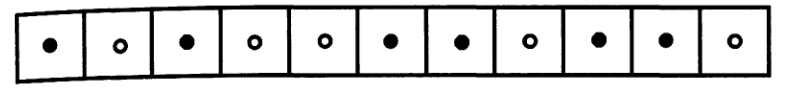
\includegraphics[width=0.7\linewidth]{img/write-05/yacheiki}
	\caption{Возможное распределение ферми-частиц по ячейкам (черная точка - ферми частица, белая точка - отсутсвие частицы)}
	\label{fig:yacheiki}
\end{figure}
Разбив систему на $Z$ ячеек, найдем количество распределений $N$ фермионов по $Z$ ячейкам, то есть статистический вес макросостояния системы фермионов
\begin{equation*}
	W = \frac{Z!}{N!(Z-N)!}
\end{equation*}

Рассмотрим шестимерное фазовое пространство с координатами $x,y,z,p_x,p_y,p_z$. Разобьем его с помощью изоэнергетических поверхностей
\begin{equation*}
	f(x,y,z,p_x,p_y,p_z) = E_i = \mathrm{const}
\end{equation*}
на тонкие слои так, что $|E_{i+1}-E_{i}|\ll E_i$. Пусть в пределы $i$-го слоя попадает $Z_i$ ячеек объемом $(2\pi\hbar)^3$ и $N_i$ частиц. Тогда аналогично примеру с раскладыванием фермионов по ячейкам получим статистический вес каждого энергетического слоя:
\begin{equation*}
	\Omega_i = \frac{Z_i!}{N_i!(Z_i-N_i)!}
\end{equation*}
Статистический вес всей системы равен произведению статистических весов её подсистем:
\begin{equation*}
	\Omega = \prod_i \Omega_i
\end{equation*}

Для нахождения наиболее вероятного распределения частиц по ячейкам, необходимо найти максимум статистического веса системы при условии, что количество частиц постоянно и полная энергия постоянна (жесткая адиабатическая оболочка), то есть
\begin{equation*}
	\sum N_i=\mathrm{const},\quad \sum E_iN_i=\mathrm{const}.
\end{equation*}

Вспомним формулу Больцмана для энтропии $S=k\ln \Omega$, вместо максимума $\Omega$ будем искать максимум энтропии. По свойствам логарифмов:
\begin{equation*}
	S=k\sum_i \big[\ln Z_i! - \ln N_i ! - \ln(Z_i - N_i)!\big]
\end{equation*}

Так как $N_i, Z_i \gg 1$, то воспользуемся формулой Стирлинга ($\ln n! \approx n\ln n - n$).
\begin{equation*}
	S=k\sum_i \big[
	Z_i \ln Z_i - Z_i - N_i \ln N_i + N_i - (Z_i-N_i)\ln(Z_i-N_i) + (Z_i-N_i)
	\big]
\end{equation*}
Слагаемое $Z_i \ln Z_i$ исключим из выражения, так как при поиске экстремума энтропии варьироваться будут только числа частиц в слое $N_i$, а данное слагаемое от них не зависит.

\textit{Метод множителей Лагранжа}. Рассмотрим функцию
\begin{equation*}
	F = S + \lambda_1 N + \lambda_2 E = -k\sum_i \big[N_i\ln N_i+(Z_i-N_i)\ln (Z_i-N_i)\big] + \lambda_1 \sum_i N_i + \lambda_2 \sum_i N_iE_i
\end{equation*}
Приравнивая к нулю частные производные $F$ по $N_i$, получаем:
\begin{equation*}
	\frac{\partial F}{\partial N_i} = -k \left[
	\ln N_i + N_i\frac{1}{N_i}-\ln(Z_i-N_i)-(Z_i-N_i)\frac{1}{Z_i-N_i}
	\right] + \lambda_1 + \lambda_2 E_i = k \ln \frac{Z_i-N_i}{N_i} + \lambda_1 + \lambda_2E_i=0
\end{equation*}
Отсюда следует, что:
\begin{equation*}
	\ln \frac{Z_i-N_i}{N_i} = -\frac{\lambda_2 E_i+\lambda_1}{k} \Leftrightarrow
	\frac{Z_i-N_i}{N_i} = \frac{1-\frac{N_i}{Z_i}}{\frac{N_i}{Z_i}}=\exp \left\{-\frac{\lambda_2 E_i+\lambda_1}{k}\right\}
\end{equation*}
Отношение $\frac{N_i}{Z_i}$ представляет собой среднее число фермионов $<n_i>$ в одной ячейке (т.е. в одном квантовом состоянии). Наиболее вероятным значением $<n_i>$, как следует из поиска экстремума, является:
\begin{equation*}
	<n_i>=\frac{1}{\exp \left\{-\frac{\lambda_2 E_i+\lambda_1}{k}\right\}+1}
\end{equation*}

Поскольку все частные производные $F$ по $N_i$ равны нулю, то равен нулю и дифференциал этой функции $dF$, то есть:
\begin{equation*}
	dF = dS + \lambda_1 dN + \lambda_2 dE = 0
\end{equation*}
Но так как число частиц системы постоянно ($\sum N_i=\mathrm{const}$), то $dN=0$, а следовательно:
\begin{equation*}
	dS + \lambda_2 dE = 0 \implies \lambda_2 = -\frac{dS}{dE}
\end{equation*}
\begin{equation*}
	\begin{cases}	
	dS \overset{\mathrm{def}}{=\joinrel=} \frac{\delta Q}{T}\\
	\delta Q = dE,\,\text{т.к.}\, V=\mathrm{const}
	\end{cases}\implies \lambda_2 = -\frac{dS}{dE} = -\frac{\delta Q}{TdE} = -\frac{1}{T}
\end{equation*}
Множитель $\lambda_1$ представим в виде $\lambda_1=\frac{\mu}{T}$, где $\mu$ - некоторая функция параметров состояния системы, в частности температуры. $\mu$ называют химический потенциал.

С учетом выражений для $\lambda_1,\,\lambda_2$, освобождаясь от индекса $i$, получаем
\begin{equation*}
	<n>_{\textsc{Ф-Д}}=\frac{1}{\exp \left\{\frac{E-\mu}{kT}\right\}+1}
\end{equation*}
распределение Ферми-Дирака. Оно определяет среднее количество фермионов, находящихся в квантовом состоянии с энергией $E$ при температуре $T$.

\begin{wrapfigure}{r}{0.5\textwidth}
	\centering
	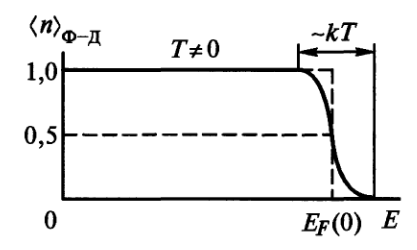
\includegraphics[width=.8\linewidth]{img/write-05/fermi-dirak-T-notzero}
	\caption{Распределение Ферми-Дирака при $T\neq 0$}
	\label{fig:fermi-dirak-t-notzero}
\end{wrapfigure}

Химический потенциал $\mu$, очевидно, имеет размерность энергии, а в случае фермионов называется \textit{энергией Ферми} или \textit{уровнем Ферми}, обозначается $E_F$.

Анализируя выражение $<n>_{\textsc{Ф-Д}}$ получим, что
\begin{align}
	T=0: <n>_{\textsc{Ф-Д}} = \begin{cases}
		1, E<E_F(0),\\
		0, E>E_F(0),
	\end{cases}
\end{align}
то есть при $T=0$ распределение принимает вид ступеньки единичной высоты, обрывающейся при $E=E_F(0)$. При $T\neq 0$ см. Рис \ref{fig:fermi-dirak-t-notzero}.
